\documentclass[12pt]{standalone}
\usepackage{tikz}
\usetikzlibrary{positioning}
\begin{document}
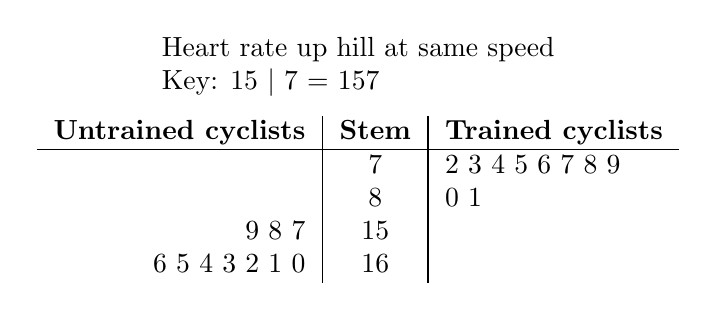
\begin{tikzpicture}
\node[align=left] (top_node) at (0,0) {Heart rate up hill at same speed \\ Key: 15 $\vert$ 7 = 157};
\node[below=of top_node,yshift=10mm] {
\begin{tabular}{r|c|l}
\textbf{Untrained cyclists} & \textbf{Stem} & \textbf{Trained cyclists}\\
\hline
 & 7 & 2 3 4 5 6 7 8 9 \\ & 8 & 0 1 \\9 8 7 & 15 &  \\6 5 4 3 2 1 0 & 16 &  \\
\end{tabular}};
\end{tikzpicture}
\end{document}